\chapter{The w-transformation} 
\label{chp:w_transformation}
\section{Introduction}
Originally, the w-transform was as a technique to perform stability analysis on discretized systems from back in the 1980s, when computational power was considerably lower. In our case, the goal is to use its similarities to the Laplace in our stability analysis. 
Although analyzing stability in the z-domain is difficult, it can be done, and some analysis of robustness can be is also possible. In this case, we will attempt to use the w-transformation in order to map the contents from within the unit-circle to the left half-plane of the w-domain. This allows for doing stability analysis there, which is much more convenient. In order to map something from the unit-circle to the left half-plane, it is possible to use a bilinear transformation, usually referred to as the w-transform. In our case, the w-transform will be used for its similarities to the s-domain, 
 hopefully giving a more accurate analysis. 

 \section{Transforming to the w-domain}
 The w-transformation is a bilinear transform that is the same as the inverse Tustin transform. 
\begin{equation}
 z = \frac{1 + \frac{T}{2}w}{1 - \frac{T}{2}w}
\end{equation}{}

\begin{equation}
 w = \frac{2}{T}\frac{z-1}{z+1}
\end{equation}{}
An important thing to note is that the bilinear transformation from the s to the z-domain is supposed to be based on $z = e^{T_s s}$, and as a result, the inverse transform should be $s = \frac{1}{T_s}\log{z}$. But, both of these transformations are impossible to perform directly, which is the reason for the simplifications. As a result, the w-domain might act very differently from how it would have acted in the s-domain. However, one feature that is preserved between both the normal and the simplified transformation is that the stability regions remain the same, even though the transformations are non-linear, even along the stability border. 

\section{Transforming matrices in the z-domain}
\label{sec:Transforming_from_z_to_w}
A system in the z-domain is usually written on the form: 
\begin{equation}
 z \Vec{x}= \Vec{A_z}\Vec{x}+ \Vec{B_z}\Vec{u}
\end{equation}
In order to transform the system properly into the w-domain, we want a system that may be on the form
\begin{equation}
 w \Vec{x}= \Vec{A_w}\Vec{x}+ \Vec{B_w}\Vec{u}
\end{equation}

But when substituting the expression for w into the expression for w into the discrete-time expression, the result is: 
\begin{equation}
 w\Vec{x} = \frac{2}{T} \left(\Vec{I} +\Vec{A_z} \right)^{-1}\left(\Vec{A_z}-\Vec{I}\right)\Vec{x} + \frac{2}{T}\left(\Vec{I}+\Vec{A}\right)^{-1}\left(\Vec{I} +\frac{Tw}{2}\Vec{I}\right)\Vec{B}\Vec{u}
\end{equation}
Now, there is an issue with the operator $w$ on the vector $\Vec{u}$. When the input is constant, there are characteristics of the s and z-transform that can be abused to get rid of the unwanted term $w\Vec{u}$. Since the operator s is the same as performing a derivative, $s\Vec{u}$ becomes 0. Whereas, z is the same as a step inot the future. But, since $\Vec{u}$ remains constant within a single step, $\Vec{u}=z\Vec{u}$. Since we have not established any similair characteristics for the w-transform, we can't transform $\Vec{u}$. Because of this, $\Vec{u}$ has to be set to be 0. Since a controller still is needed, the only solution is to describe the control law in the system matrix in the z-domain, and then use the simplified transformation. 
\begin{equation}
 w\Vec{x} = \Vec{A_w}x = \frac{2}{T} \left(\Vec{A_z} + \Vec{I}\right)^{-1}\left(\Vec{A_z}-\Vec{I}\right)\Vec{x}
\end{equation}
Or, even simpler: 
\begin{equation}
 \Vec{A}_w = \frac{2}{T} \left(\Vec{I} - 2( \Vec{I}+\Vec{A}_z)^{-1}\right)
\end{equation}{}
One of the big advantages of how this transformation has been performed is that all cotineous states in the s-domain correspond to the same states in the w-domain and all internal states in the discrete controller correspond to the same state in the w-domain. 

Also, as a reader, one might be skeptical about the fact that the inverse of $\left( \Vec{A_z} \pm \Vec{I}\right)$ is used. But, remember that the controller in the z-domain is supposed to stabilize the system. If $\left( \Vec{A_z} \pm \Vec{I}\right)$ does not have full rank, then that means that the closed-loop has at least one eigenvalue equal to 0, resulting in a marginally stable system. If that is the case, the system is either overparameterized or not robust at all. In these cases, the system is so close to unstable, that the analysis that will be given in \cref{chp:new_findings} almost never be able to guarantee any form of stability. 

\section{Some intuition}
\begin{figure}
 
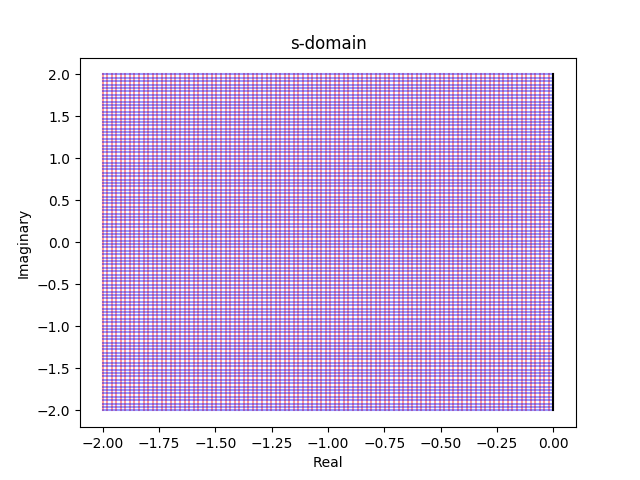
\includegraphics{Figures/s_grid.png}
 \caption{A grid in the s-domain}
 \label{fig:s_grid}
\end{figure}{}
\begin{figure}
 \centering
 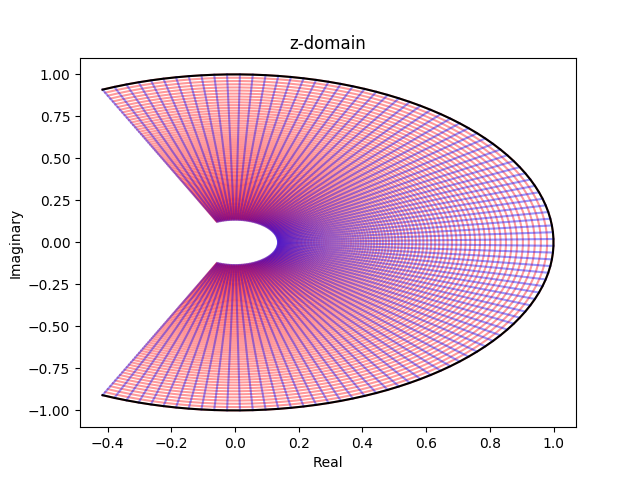
\includegraphics{Figures/z_grid.png}
 \caption{The same grid in the z-domain, sampled with a sampling period of 1 time-unit. The black line on the right side is the stability-border}
 \label{fig:z_grid}
\end{figure}{}


\begin{figure}
 \centering
 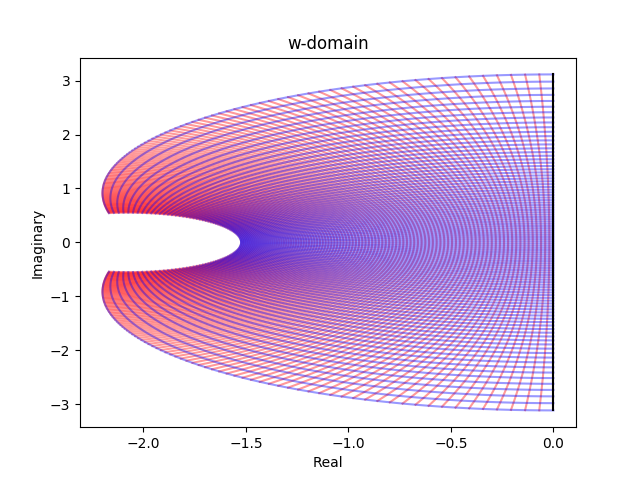
\includegraphics{Figures/w_grid.png}
 \caption{Grid in w-domain, with a sampling period of 1 time-unit}
 \label{fig:w_grid}
\end{figure}{}
As shown in \cref{fig:s_grid} and \ref{fig:w_grid}, there can be quite a bit of distortion between the s-domain and the w-domain. But the differences are rather small for poles closer to the origin. So, intuitively, the w-domain behaves more like the s-domain when the system gets closer to the stability-border, which should hopefully make it more suited for stability-analysis. 

In order to prove that the stability regions are what we say they are, we will have to do some substitutions. First, since $z = e^{s T_s}$, the only requirement is to divide it into two and observe that 
\begin{equation}
 z = e^{\Re{(s )T_s}}e^{\Im{(s )T_s}}
\end{equation}{}
Since an imaginary exponent does not change the absolute value, only the complex angle, the real part of s directly translates to the amplitude of z. Real parts less than 0, gives amplitudes less than 0. This means that the stability region will be inside the unit circle. 


Similarly, $z$ can be represented as $z = r\cdot e^{j\Theta}$. If it is put into the equation for $w$, the resulting expression becomes:

\begin{equation}
 w = \frac{2}{T}\frac{r e^{j \Theta}-1}{re^{j \Theta}+1}
\end{equation}{}
After using Euler's formula, we get: 
\begin{equation}
 w = \frac{2}{T_s} \frac{(r^2 -1) + j( 2\sin{\Theta}) }{1+ r^2 + 2r \cos{\Theta}}
\end{equation}{}

Since the denominator is real, the real part of $w$ is described entirely by $\frac{r^2-1}{1+r^2 + 2 r cos (\Theta)}$. As a result, when $r<1$, then $\Re{(w)} < 0$. Also, worth noting is that as long as $\Theta =0$, the $w$ will never go beyond $-\frac{2}{T_s}$. This means that purely real eigenvalues will never go beyond the Nyquist-frequency, even though they may have faster dynamics in the s-domain. Also, if $\Theta =\frac{\pi}{2}$, and $r=1$, then, the denominator will be equal to 0. By L'Hôpital's rule, the resulting amplitude will be $\infty$. This means that oscillations near the Nyquist-frequency will potentially be mapped far away from where a similar point would have been in the s-domain. This helps to highlight one of the weaknesses of the w-transform. If a mode is very close to the Nyquist-frequency if will become more difficult to analyze. But preferably, all modes that might cause instability should be below the Nyquist-frequency. But, in practice, in order to avoid the issues of sampling, it is normal to have a sampling-rate that is between $\frac{1}{2}$ and $\frac{1}{5}$ of the Nyquist-frequency. The advantages of a high sampling-frequency can be seen in \cref{fig:dif_s_and_w}. As a result of the high sampling-rate, the differences will usually not be that large.


\begin{figure}
 \centering
 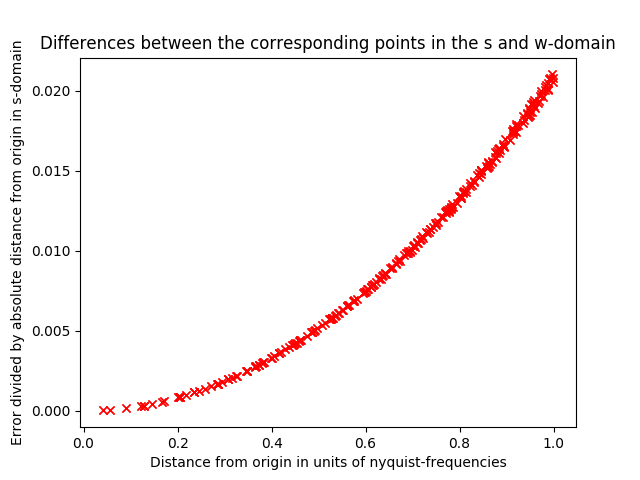
\includegraphics{Figures/differences_in_well_behaved_region.png}
 \caption{The difference between a point in the s-domain and in the w-domain is quite good below the Nyquist-frequency, but becomes worse quickly}
 \label{fig:dif_s_and_w}
\end{figure}
\todo[inline]{Nyquist ofte mellom 1/5 og maks til 1/2 av Nyquist (eller 1/10 og 1/20)}
\noindent

Finally, the last useful characteristic of the w-transform is that, unlike the z-transform, the placement of the poles are not as affected by the sampling-frequency as the z-transform. In the z-transform, a pole at $\lambda_i$, at a sampling-period $T_s$, will be mapped to the same point as a pole at $2\lambda_i$ if the sampling-period is halved to $\frac{T_s}{2}$. As long as the sampling-rate is so high that a pole is within the somewhat linear part of the w-domain, it will not change a position based on the sampling-frequency. This may make the analysis a bit more intuitive. 